% =====================================================================
%  N7: roadmap.
%  Sources: openhydroqual.com "What's next", codegen/README.md remaining
%  work, and the OpenHydroTwin streaming-MCMC work in progress.
%  Build: pdflatex fig_roadmap.tex && cp fig_roadmap.pdf figures/N7_roadmap.pdf
% =====================================================================
\documentclass[border=4pt]{standalone}
\usepackage[T1]{fontenc}
\usepackage{helvet}
\renewcommand\familydefault{\sfdefault}
\usepackage{tikz}
\usetikzlibrary{arrows.meta,positioning,calc,fit,backgrounds}

\definecolor{ohqblue}{HTML}{1F5C8B}
\definecolor{ohqteal}{HTML}{2A9D8F}
\definecolor{ohqsand}{HTML}{E9C46A}
\definecolor{ohqrust}{HTML}{E76F51}
\definecolor{ohqgrey}{HTML}{6B7280}
\definecolor{bandfill}{HTML}{EDF1F4}

\begin{document}
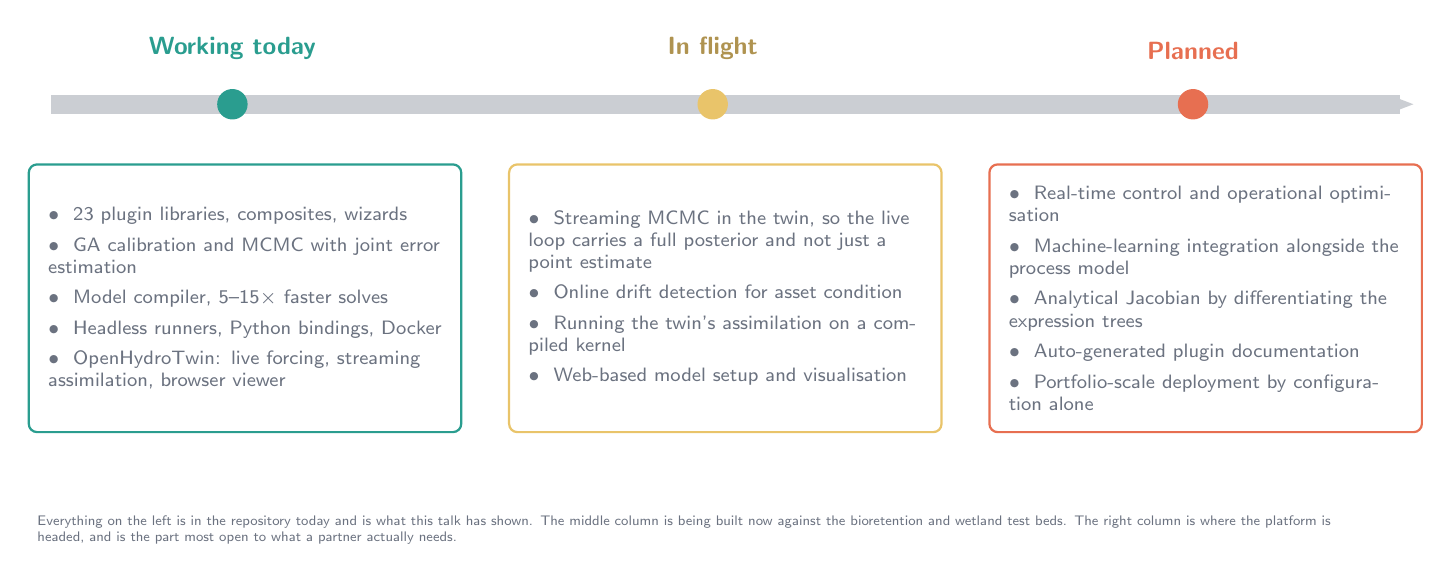
\begin{tikzpicture}[
  font=\sffamily,
  card/.style={draw=ohqgrey!45, line width=0.8pt, fill=white, rounded corners=3pt,
               align=left, inner sep=7pt, font=\scriptsize, text=ohqgrey,
               text width=50mm, minimum height=34mm, anchor=north west},
  hdr/.style={font=\small\bfseries, anchor=west},
  lbl/.style={font=\tiny, text=ohqgrey, align=left},
]

% ---------------- the spine -----------------------------------------
\draw[-{Stealth[length=8pt]}, ohqgrey!35, line width=7pt]
  (-0.4,0) -- (16.9,0);

\foreach \x/\c in {1.9/ohqteal, 8.0/ohqsand, 14.1/ohqrust}
  \fill[\c] (\x,0) circle (5.5pt);

\node[hdr, text=ohqteal, anchor=south] at (1.9,0.45) {Working today};
\node[hdr, text=ohqsand!75!black, anchor=south] at (8.0,0.45) {In flight};
\node[hdr, text=ohqrust, anchor=south] at (14.1,0.45) {Planned};

% ---------------- cards ---------------------------------------------
\node[card, draw=ohqteal] (c1) at (-0.7,-0.75) {%
  $\bullet$~~23 plugin libraries, composites, wizards\\[3pt]
  $\bullet$~~GA calibration and MCMC with joint error estimation\\[3pt]
  $\bullet$~~Model compiler, 5--15$\times$ faster solves\\[3pt]
  $\bullet$~~Headless runners, Python bindings, Docker\\[3pt]
  $\bullet$~~OpenHydroTwin: live forcing, streaming assimilation, browser viewer};

\node[card, draw=ohqsand] (c2) at (5.4,-0.75) {%
  $\bullet$~~Streaming MCMC in the twin, so the live loop carries a full
  posterior and not just a point estimate\\[3pt]
  $\bullet$~~Online drift detection for asset condition\\[3pt]
  $\bullet$~~Running the twin's assimilation on a compiled kernel\\[3pt]
  $\bullet$~~Web-based model setup and visualisation};

\node[card, draw=ohqrust] (c3) at (11.5,-0.75) {%
  $\bullet$~~Real-time control and operational optimisation\\[3pt]
  $\bullet$~~Machine-learning integration alongside the process model\\[3pt]
  $\bullet$~~Analytical Jacobian by differentiating the expression trees\\[3pt]
  $\bullet$~~Auto-generated plugin documentation\\[3pt]
  $\bullet$~~Portfolio-scale deployment by configuration alone};

\node[lbl, anchor=north west, text width=168mm] at (-0.7,-5.1)
  {Everything on the left is in the repository today and is what this talk has
   shown. The middle column is being built now against the bioretention and
   wetland test beds. The right column is where the platform is headed, and is
   the part most open to what a partner actually needs.};

\end{tikzpicture}
\end{document}
